%%____________________________________________________________________________||
\section{Systematic uncertainties in background estimation}
\label{sec:systematics}

This section addresses the estimation of systematic uncertainties
associated with the predictions of the non-multijet backgrounds. Since
this analysis aims to rely as much as possible on the data control
samples to check for sources of bias and derive and/or cross check
systematic uncertainties, a detailed study can only be meaningfully
carried out with data. The strategies that will be employed to
ascertain the presence of biases or otherwise, and the procedures used
to derive systematic uncertainties, are described below. The MC-based
expectations for uncertainties in the background predictions under the
assumption of zero bias (\ie, only the statistical component) are
presented. The assumptions made in the projections of physics reach
that are detailed in Section \ref{sec:susy} are also outlined.

Two types of systematic uncertainty are considered separately. First,
the normalisation uncertainties affect the background predictions for
the signal region in each (\nb,\njet,\scalht) bin (integrated over \mht)
These uncertainties are estimated with closure tests, described in
Sections~\ref{sec:bkgdnorm-syst} and \ref{sec:syst-from-closure}.

Second, systematic effects that may result in the migration of
(simulated) events between \mht bins within a given (\njet,\nb,\scalht)
bin is accounted for by providing alternative templates to the nominal
\mht template obtained from simulation. These alternative \mht
templates may be derived from, or at least cross checked with, the
data control samples, as described in Section~\ref{sec:syst-on-shape}.

% % Maybe we can re-use this table at some point
% \begin{table}[h!]
%   \caption{Systematic uncertainties on the transfer factors as a
%     function of \scalht.}  
%   \label{tab:bkgd-syst}
%   \setlength{\extrarowheight}{2.5pt}
%   \centering
%   \begin{tabular}{ llccc }
%     \hline
%     \hline
%     \scalht region [GeV] & 200-600 & 600-1000  & $>1000$  \\ 
%     \hline
%     Uncertainty [\%] & 10 & 20 & 30 \\
%     \hline
%     \hline
%   \end{tabular}
% \end{table}
%
% The uncertainties associated with the b-tag ``fomula method'' used
% during Run~1 are ascertained through a dedicated procedure and are
% assumed to be sub-dominant with respect to the \scalht-dependent
% uncertainties derived from the closure tests, as observed during
% Run~1. 
%\clearpage

\subsection{Closure tests}
\label{sec:closure-tests-desc}
\label{sec:bkgdnorm-syst}

The background estimates are determined in each (\nb,\njet,\scalht) bin by
defining transfer factors from control region to signal region, as
described in Section \ref{sec:selection}. Since the transfer factors
are obtained from simulation, an appropriate systematic uncertainty is
assigned to each transfer factor to account for limitations in the
simulation modelling of event kinematics and instrumental effects. The
next two sections describe how the systematic uncertainties are
determined from closure tests in data.

The sensitivity of the transfer factors to potential limitations in
the simulation modelling is established through sets of closure tests,
which confront data yields measured in one data control (sub-)sample
against the predictions determined from another data control
(sub-)sample as a function of \scalht. \ie, an extrapolation is made
from one control (sub-)sample to another (rather than to the signal
region) in bins of \scalht via appropriate transfer factors, again
determined from simulation. A large ensemble (\ie hundreds) of
statistically independent closure tests are performed between a number
of control (sub-)samples to identify any potential sources of bias in
the transfer factors.

The level of statistical consistency between the predicted and
observed yields of each closure test in the ensemble is inspected, in
the absence of any bias in the transfer factors. The level of
agreement between the predicted and observed yields is expressed as
the ratio $(\nobs - \npre)/\npre$ while considering only the
statistical uncertainties on \npre and \nobs. Therefore, the level of
closure is defined by the statistical significance of a deviation in
the ratio from zero. A set of closure tests comprise ratios determined
for each \scalht bin. In this way, a set of closure tests allow to
establish the presence of significant biases or otherwise, and any
possible dependence on \scalht. If statistically significant biases
are observed, further studies are required to understand and correct
for these biases.

Under the assumption of closure for the full ensemble of tests,
systematic uncertainties on the transfer factors are derived for each
\njet and \nb category and \scalht bin. The treatment for
estimating the systematic uncertainties on the transfer factors is
described in Section~\ref{sec:syst-from-closure}.

Thirteen sets of closure tests use the five data control samples to
probe key ingredients of the simulation modelling of the SM
backgrounds with genuine \met as a function of \scalht. These are
shown in Fig.~\ref{fig:closure} for both 3 \ifb and 10 \ifb and two
different jet multiplicity bins: $\njet = 4$ and $\geq 5$. In the case
that there are no statistics in a control region (sub-)sample to 
perform one of the closure tests, a red band is drawn. In these
instances, the bin in question would not be used in the statistical
interpretation of the analysis.

%create mode 100644 notes/AN-15-004/trunk/figures/closureTests/summary_plots10fb.pdf
%create mode 100644 notes/AN-15-004/trunk/figures/closureTests/summary_plots1fb.pdf
%create mode 100644 notes/AN-15-004/trunk/figures/closureTests/summary_plots3fb.pdf
%create mode 100644 notes/AN-15-004/trunk/figures/closureTests/systOut2d10fb.pdf
%create mode 100644 notes/AN-15-004/trunk/figures/closureTests/systOut2d1fb.pdf
%create mode 100644 notes/AN-15-004/trunk/figures/closureTests/systOut2d3fb.pdf
\begin{figure}[h!]
  \begin{center}
    \subfigure[Legend]{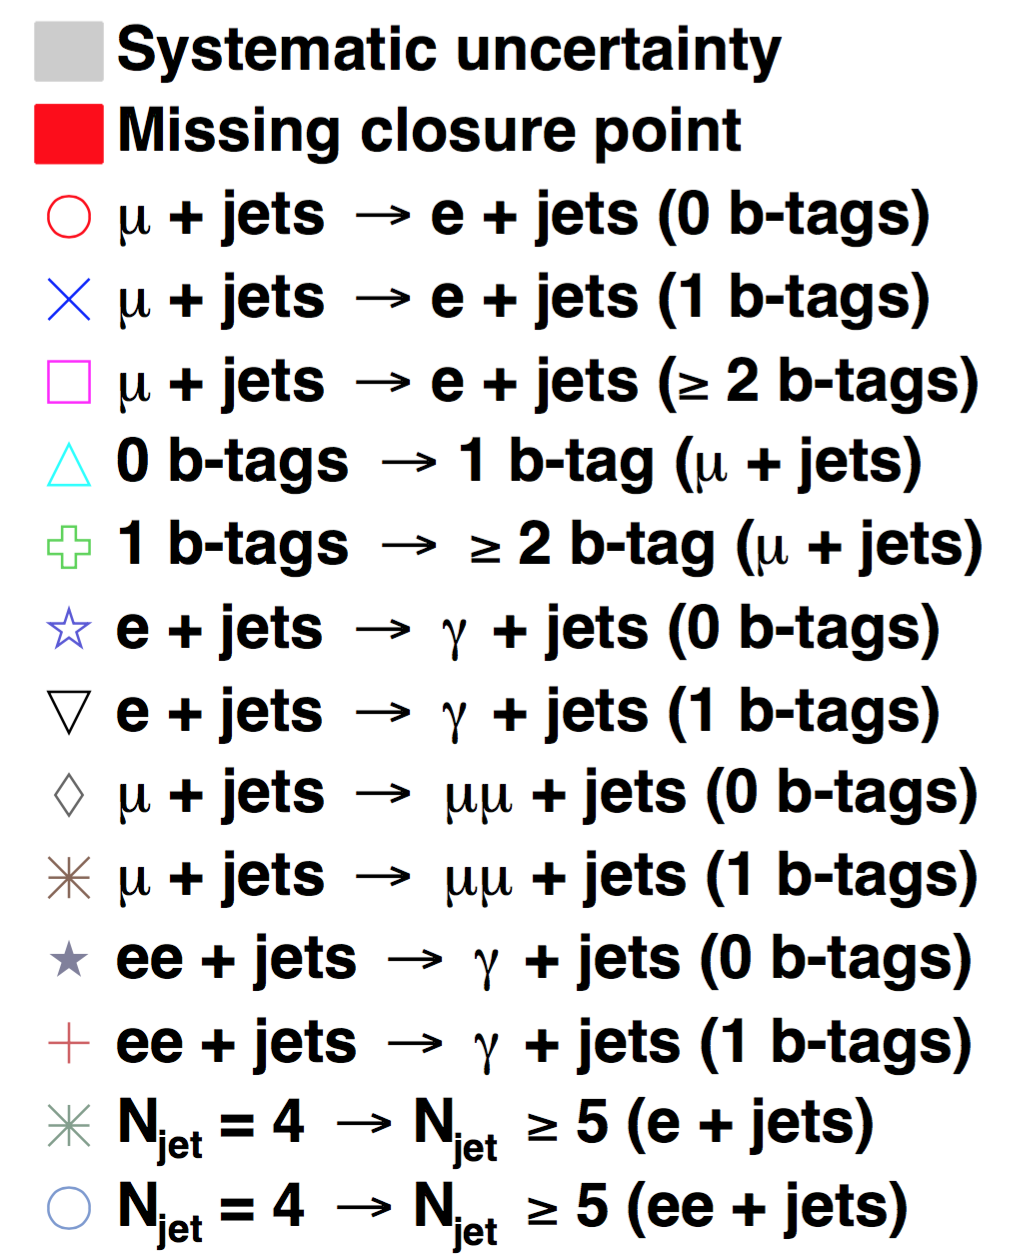
\includegraphics[width=0.3\textwidth]{figures/closureTests/legend.png}} \\
    \subfigure[$L_{\rm int} = 3\fbinv, \njet = 4$]{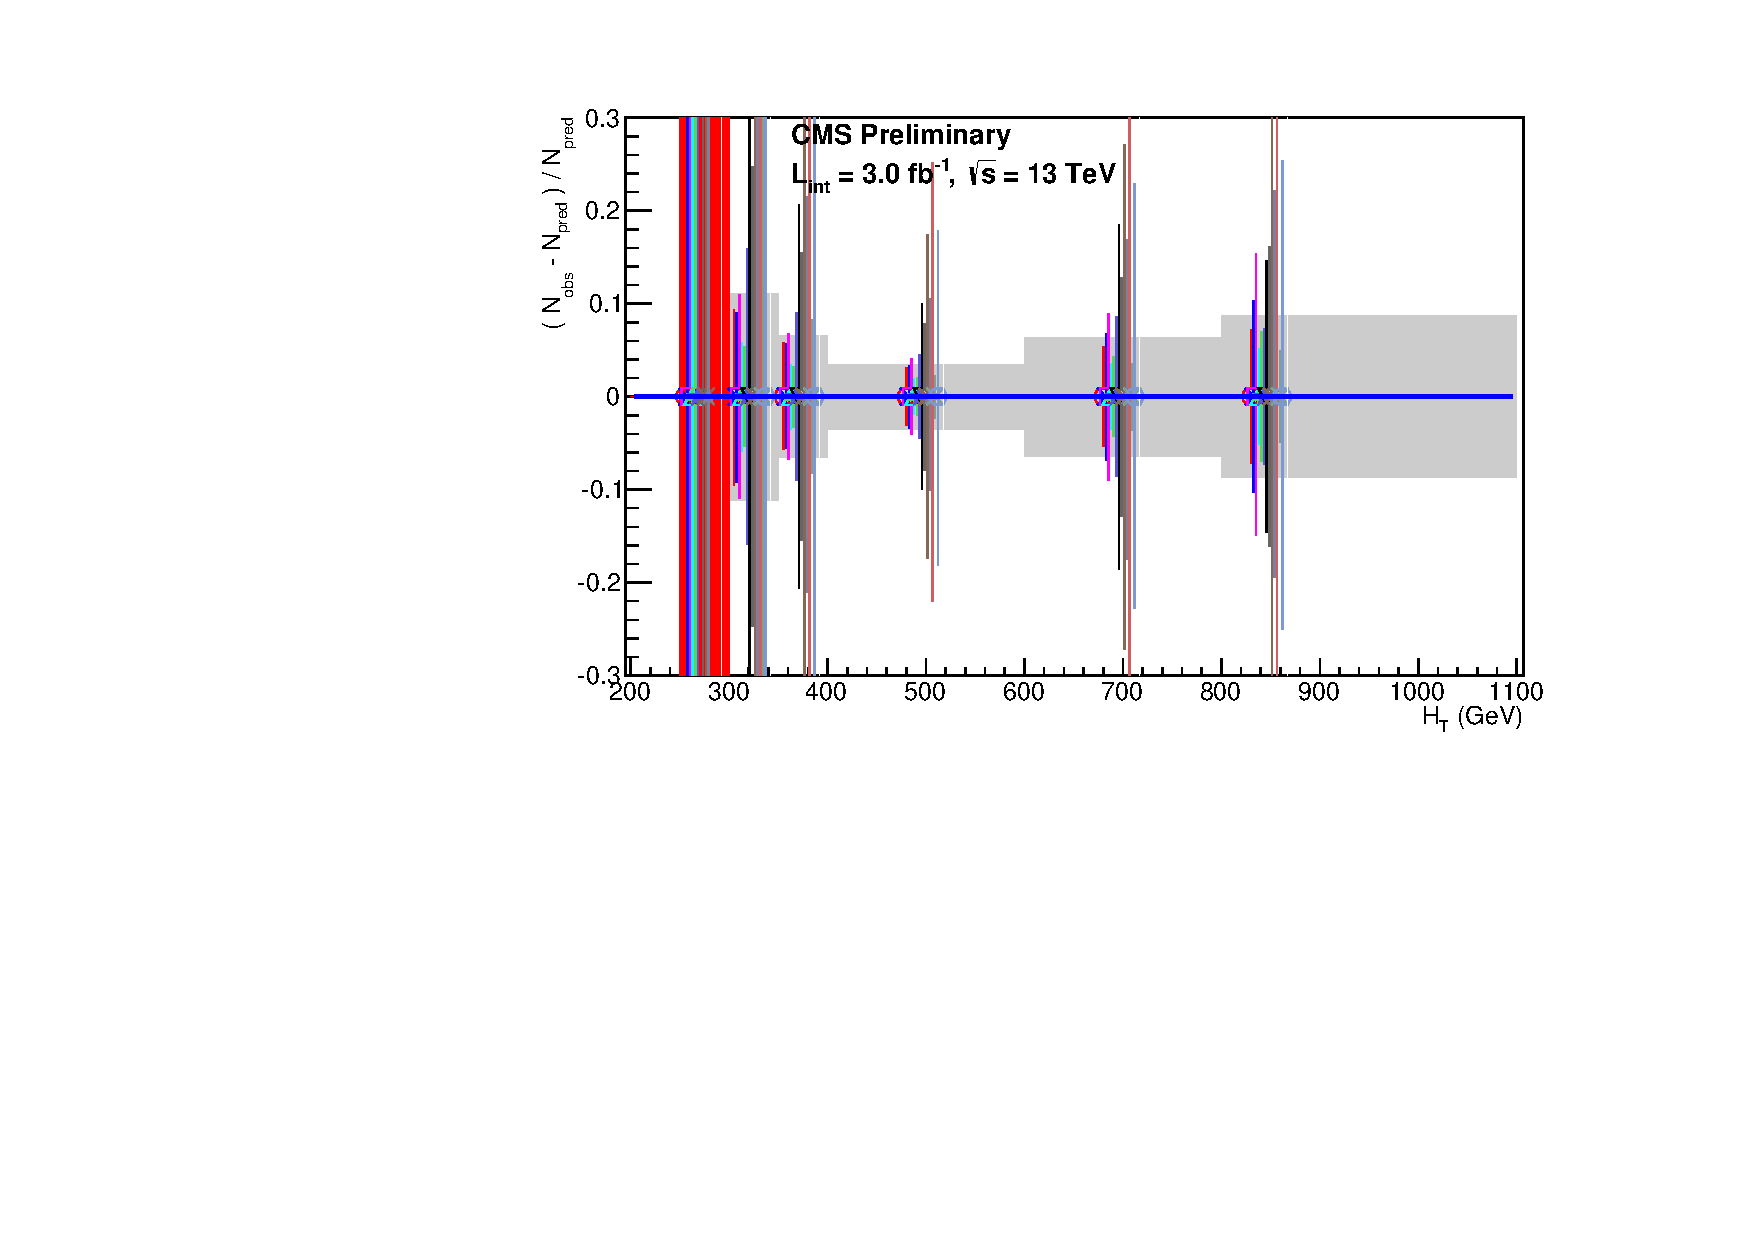
\includegraphics[width=0.5\textwidth]{figures/closureTests/eq4j_htClosure_3fb.pdf}} ~~
    \subfigure[$L_{\rm int} = 3\fbinv, \njet \geq 5$]{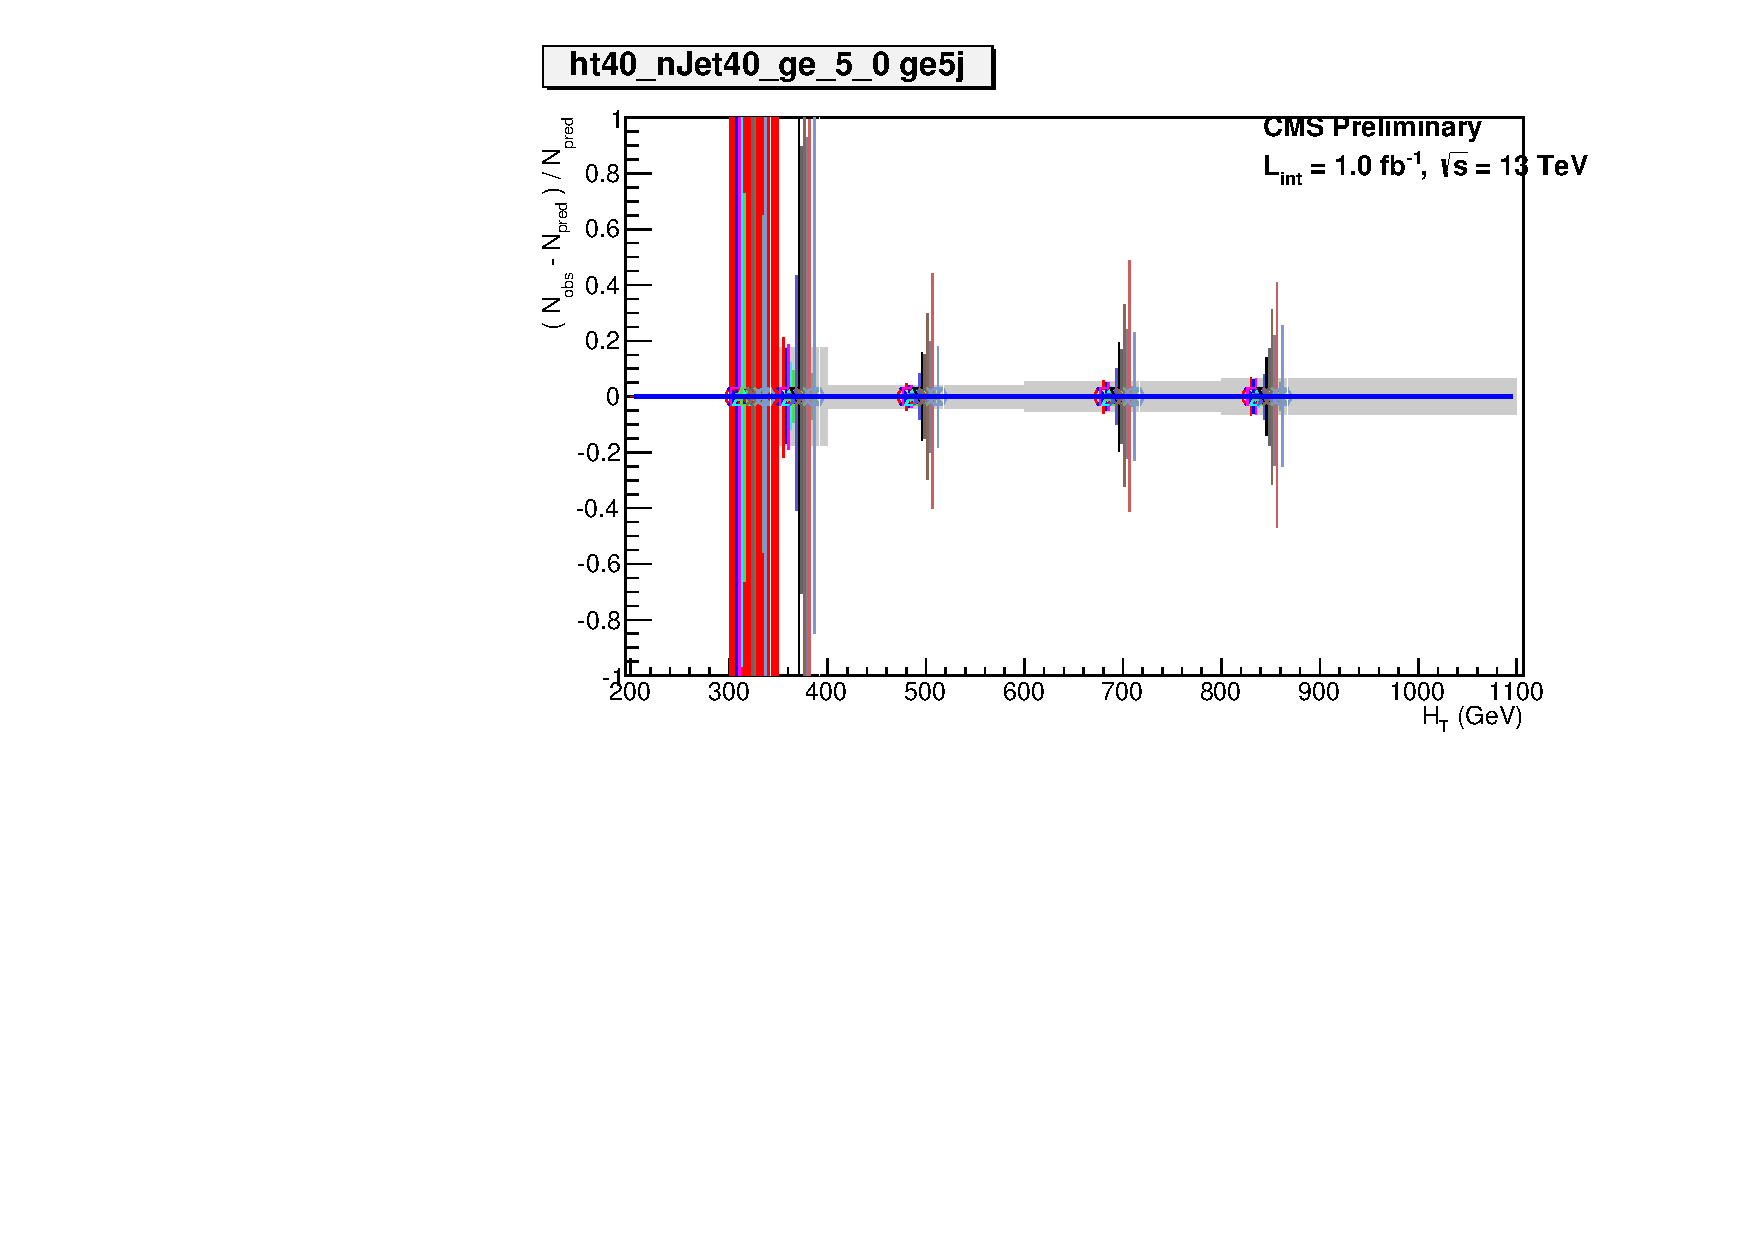
\includegraphics[width=0.5\textwidth]{figures/closureTests/ge5j_htClosure_3fb.pdf}} \\
    \subfigure[$L_{\rm int} = 10\fbinv, \njet = 4$]{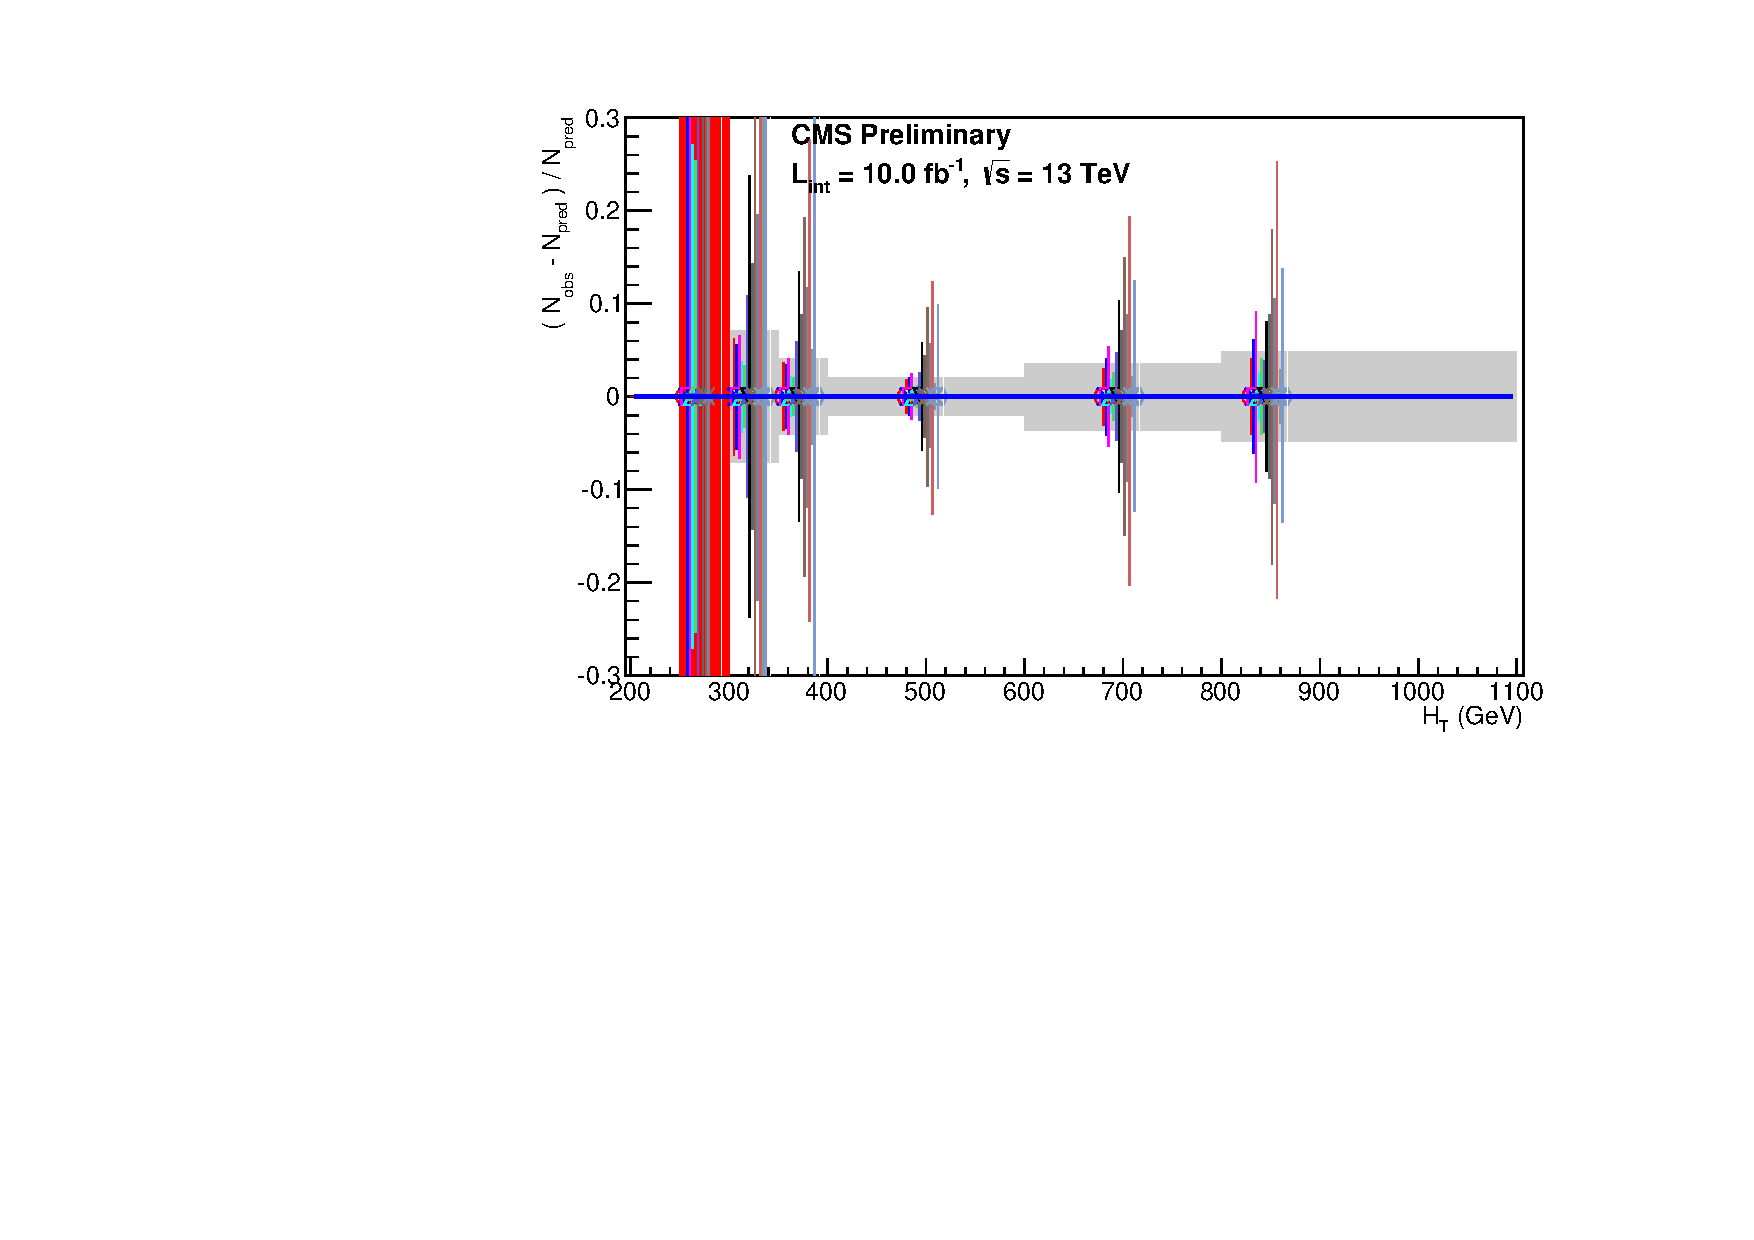
\includegraphics[width=0.5\textwidth]{figures/closureTests/eq4j_htClosure_10fb.pdf}} ~~
    \subfigure[$L_{\rm int} = 10\fbinv, \njet \geq 5$]{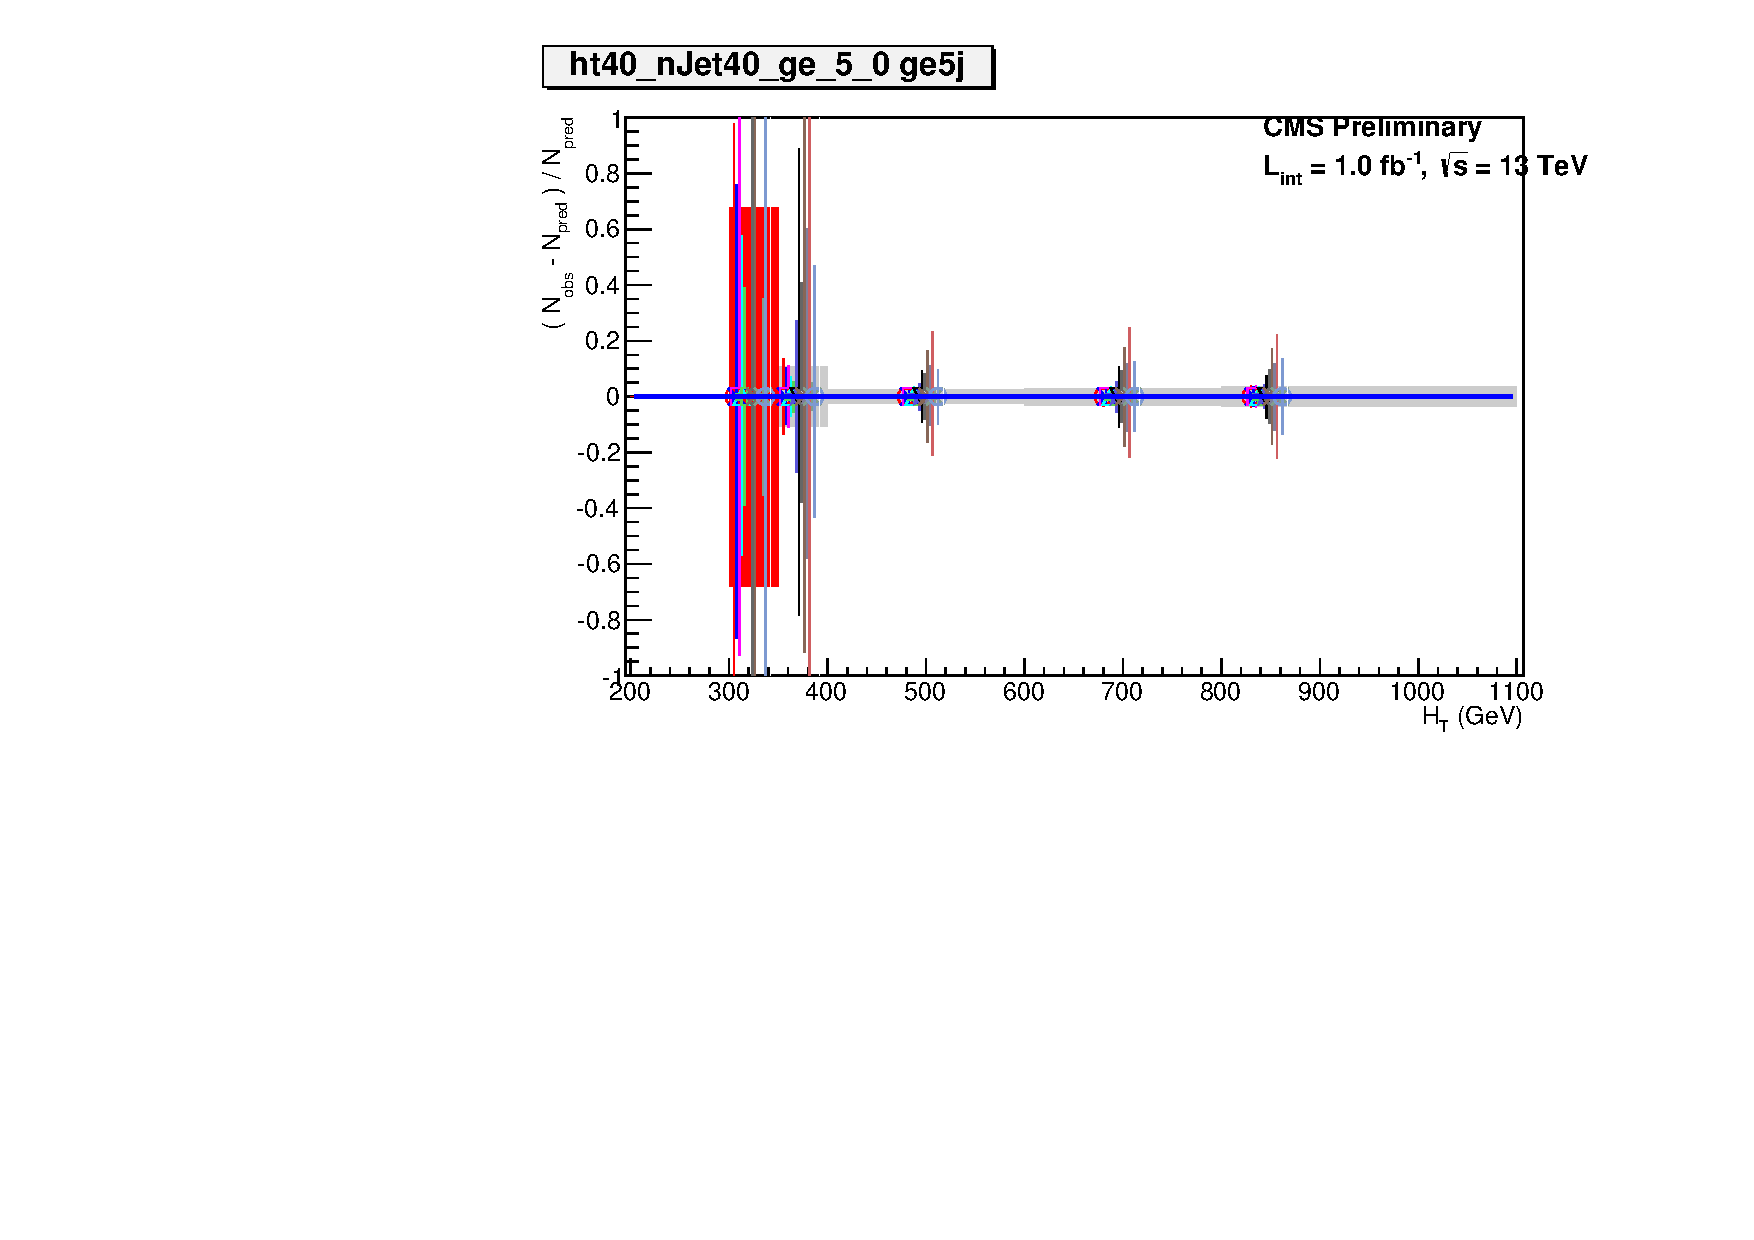
\includegraphics[width=0.5\textwidth]{figures/closureTests/ge5j_htClosure_10fb.pdf}} \\
    \caption{Sets of closure tests (open symbols) overlaid on top of
      the systematic uncertainty estimates used for each of the seven
      \scalht bins (shaded bands), for two different integrated
      luminosity scenarios (rows) and for two different jet
      multiplicity bins (columns).}
    \label{fig:closure}
  \end{center} 
\end{figure}

The first three sets of closure tests are carried out between the \mj
sample and the \ej sample. These cross check the two different lepton
identification efficiencies for three b-tag multiplicity scenarios,
\njet = 0 (red circles), 1 (times symbols) and $\geq$2 (squares).
%% In particular, the 0 b-tag sub-sample is enriched in $W$+jets events, while the $\geq$2 b-tags is very pure in \ttbar.
% The first three sets of closure tests are carried out within the $\mu$
% + jets sample. The first set (indicated by circles) probes the
% modelling of the \alphat distribution in genuine \met events as a
% function of \scalht. This is important to verify the approach of using
% \mj and \mmj samples without an \alphat requirement to make background
% predictions in the signal region, as described in
% Sec.~\ref{sec:larger}. The tests confront data yields in the \mj
% sample with an \alphat requirement against predictions determined in a
% \mj sample with the \alphat requirement inverted. As usual,
% corresponding expectations from simulation are obtained to construct
% the transfer factors required to make the predictions.

The fourth (triangles) and fifth (green crosses) sets probe the
sensitivity of the transfer factors to the relative admixture of
events from the $W$ + jets and \ttbar processes by varying the number
of b-tagged jets within the \mj sample. These tests are conservative,
as the admixture changes little between the \mj sample and the signal
region (as there is no extrapolation in \nb), whereas the closure
tests use sub-samples with different \nb bins and therefore different
admixtures of $W$ + jets and \ttbar events. \eg, the former uses a
W-enriched sub-sample (selected by requiring zero b-jets) to predict
yields in a \ttbar-enriched sub-sample (selected by requiring one
b-jet).  These two tests also probe the modelling of the
reconstruction of b-quark jets, although this is addressed more
precisely by dedicated studies involving varying the uncertainties in
b-tag scale factors, as the one performed in the previous analysis,
see for instance \cite{CMS_AN_2013-366}. This study will be repeated
for this analysis.

The sixth (hollow stars) and seventh (inverse triangles) set deal with
the consistency of the prediction of \wej with $\gamma$ + jets in two
different b-tag multiplicity bins. This is important for understanding
the consistency of the \znunu + jets background predictions from both
\wej events and the \gj process and the associated assumptions (such
as the negligible effect of the vector boson mass on kinematic
distributions from the V + jets and \gj samples under sufficient
boost). Additional checks between these two sub-samples (and also
between the single and di-lepton sub-samples) will also be performed
with the charge of the single lepton sample taken into consideration,
which will allow to probe the simulation modelling of acceptance
effects due to W polarisation.

The eighth (diamonds) and ninth (brown asterisks), connecting the $\mu$
+ jets and $\mu\mu$ + jets control samples for two different \nb bins
(zero and one) addresses the modelling of vector boson production
(including the handling of contamination from \ttbar). The muon
trigger and reconstruction efficiencies are also probed, given that
exactly one and two muons are required in the two control
samples. However, dedicated data-driven methods are used to measure
the muon trigger and reconstruction efficiencies, with values taken
from the muon POG.

The tenth (solid stars) and eleventh (red crosses) deal with the
consistency between the \zee + jets and $\gamma$ + jets
samples, which is a further check on the validity of using the \gj
process to predict the \znunu\, + jets process.

The twelfth, and thirteenth tests probe the simulation modelling of
jet multiplicity in the \ej (green asterisks), and \eej (blue circles),
which is checked due to the exclusive binning in jet multiplicity.  As
in the case of the $W$ + jets / \ttbar admixture, this set of tests is a
very conservative check, as predictions are always made from the same
jet multiplicity bin, whereas the closure tests translate between the
two bins.

The aforementioned closure tests are not the only ones considered or
checked, \ie, the list above is not exhaustive. However, they are a
representative set that cover the main potential sources of bias in
the transfer factors derived from simulation. 

Each set of closure tests should demonstrate {\bf in data}, within the
statistical precision of each test, that there are no significant
biases or dependencies on \njet nor \scalht inherent in the transfer
factors obtained from simulation. The MC-based studies shown above
close by construction, but provide information on the precision at
which biases can be probed, \ie they provide lower bounds on the
systematic uncertainties that can be derived (described below), which
can be interpreted as a systematic uncertainty limited by statistical
uncertainties associated with the data (and simulation).

Prior to deriving uncertainties, each individual set of closure tests
(as a function of \scalht) is inspected for closure. Zero and first order
polynomial fits are performed along the \scalht dimension for each set
of closure tests per jet category. The fits will be inspected for any
indication of bias averaged over \scalht as well as any
\scalht-dependant bias.

\subsection{Systematic uncertainties in the transfer factors\label{sec:syst-from-closure}}

Once it is established that no significant bias or trend is observed
for any set of closure tests, the systematic uncertainties associated
with the transfer factors are determined. The statistical precision of
the closure tests is considered a suitable benchmark for determining
the systematic uncertainties that are assigned to the transfer
factors, as it is only the statistical uncertainties associated with
the tests that limit our knowledge of whether closure is actually
achieved or otherwise.

The systematic uncertainties in the transfer factors can be considered
as a ``normalisation'' uncertainty in the SM background predictions,
which are determined per \scalht bin per (\njet,\nb) category and are
assumed to be fully uncorrelated between the different (\njet,\nb)
categories and \scalht bins. Further details are provided in Section
\ref{sec:likelihood}. 

The systematic uncertainty is estimated by taking the quadrature sum
of the weighted mean and (square root of) sample variance for the
closure tests within the given \scalht bin. To find ``expected
systematics'', \nobs and \npre are taken from the same Monte Carlo
(that guarantees closure) but the statistical errors are from the
unweighted and weighted counts respectively. The expected systematic
uncertainty is then taken as the weighted mean of the error on the
closure tests. This is an estimator of the expected variance assuming
no bias that should be found in data. 

This procedure yields the values quoted in
Figure~\ref{fig:systematics}, which shows the systematic uncertainty
on the transfer factor as a function of the \scalht and (\nb,\njet)
category, extracted for two integrated luminosity scenarios: 3 \ifb
and 10 \ifb. A clear dependence on integrated luminosity is a
reflection of the fully statistical nature of the ``systematic'' in
the absence of bias. A missing entry implies that the statistics were
insufficient to complete the necessary set of closure tests and the
\scalht bin is not used for this (\njet,\nb) category. In addition to
the zero and first order polynomial fits mentioned above, a comparison
of the magnitude of the systematic found in data with that expected
from simulation (\ie in the absence of bias) will provide an
additional indication of any genuine bias.

\begin{figure}[]
  \centering
  \subfigure[Systematic uncertainties for 3 \ifb]{
    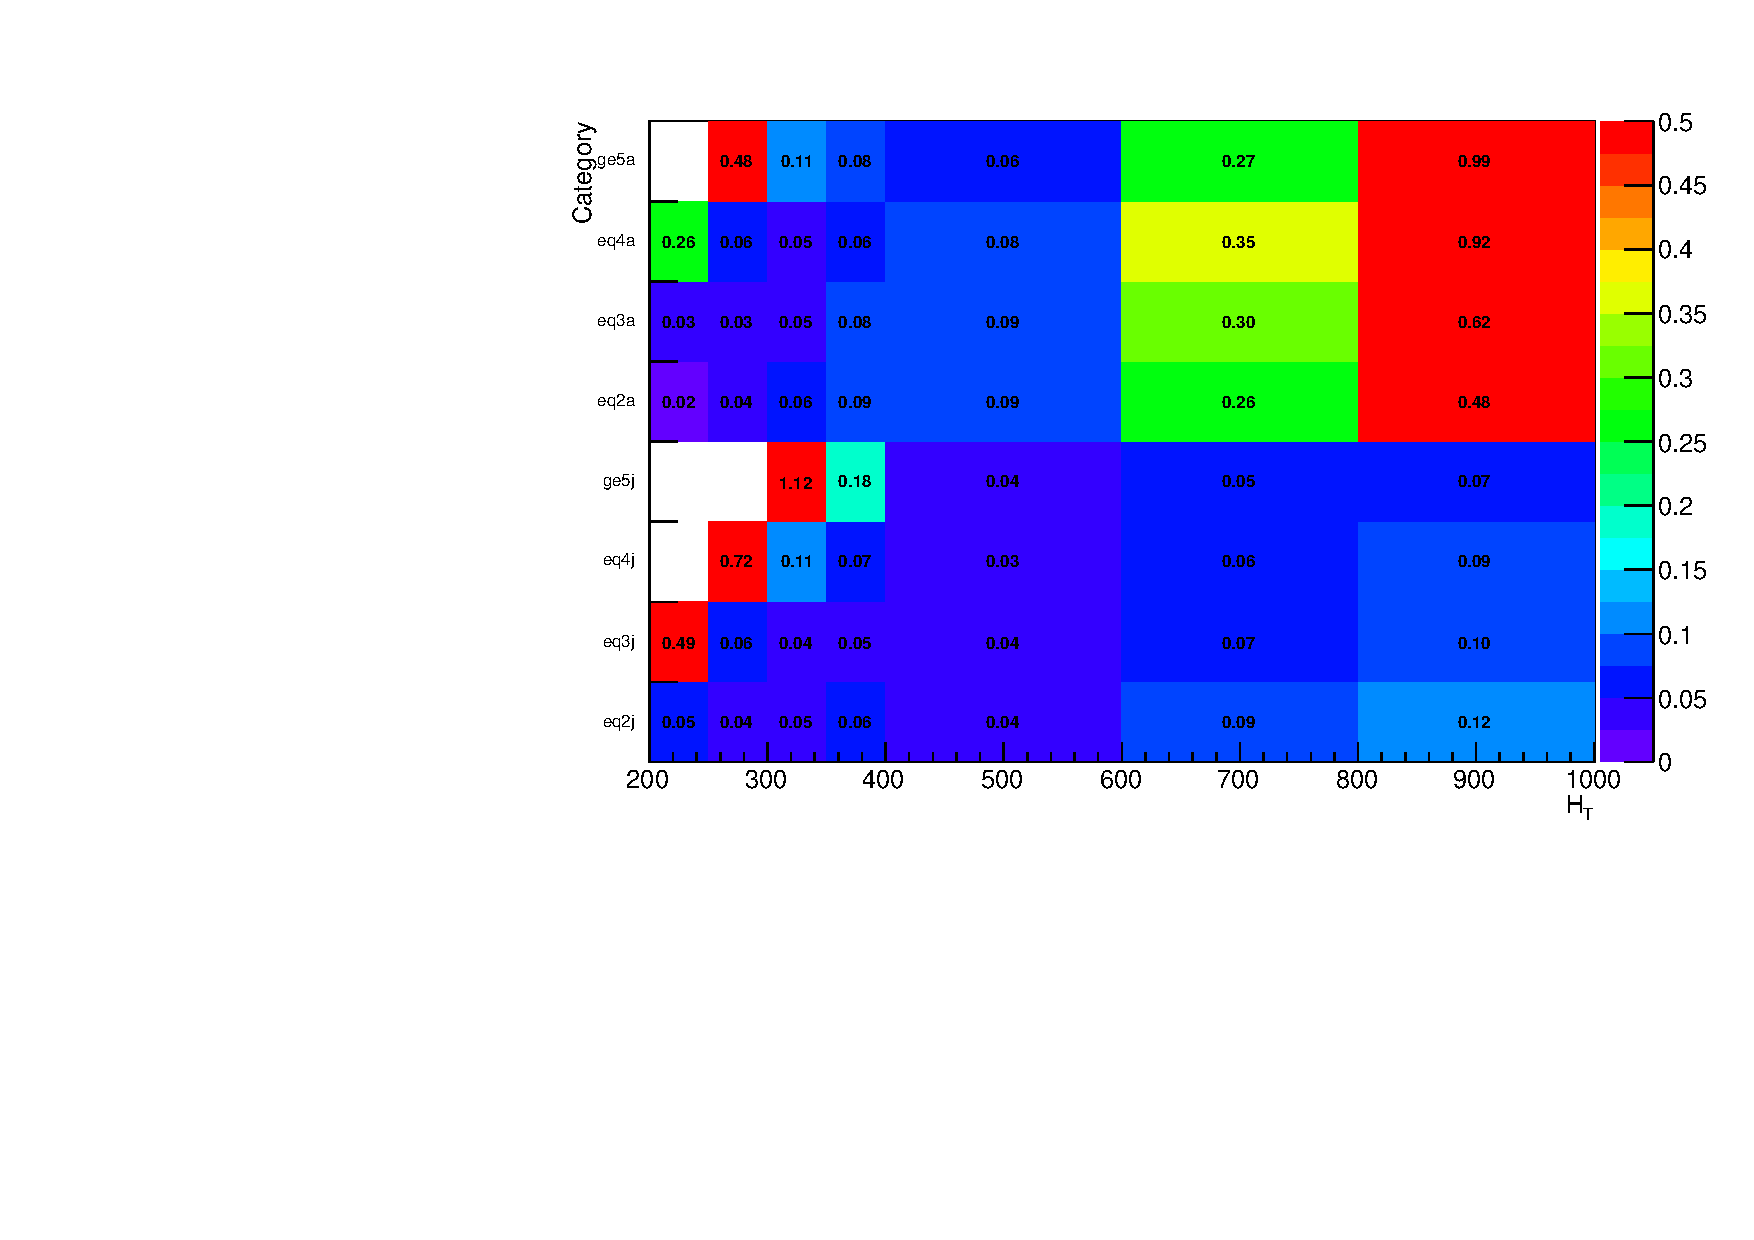
\includegraphics[width=0.5\textwidth]{figures/closureTests/systOut2d3fb.pdf}
  } ~~
  \subfigure[Systematic uncertainties for 10 \ifb]{
    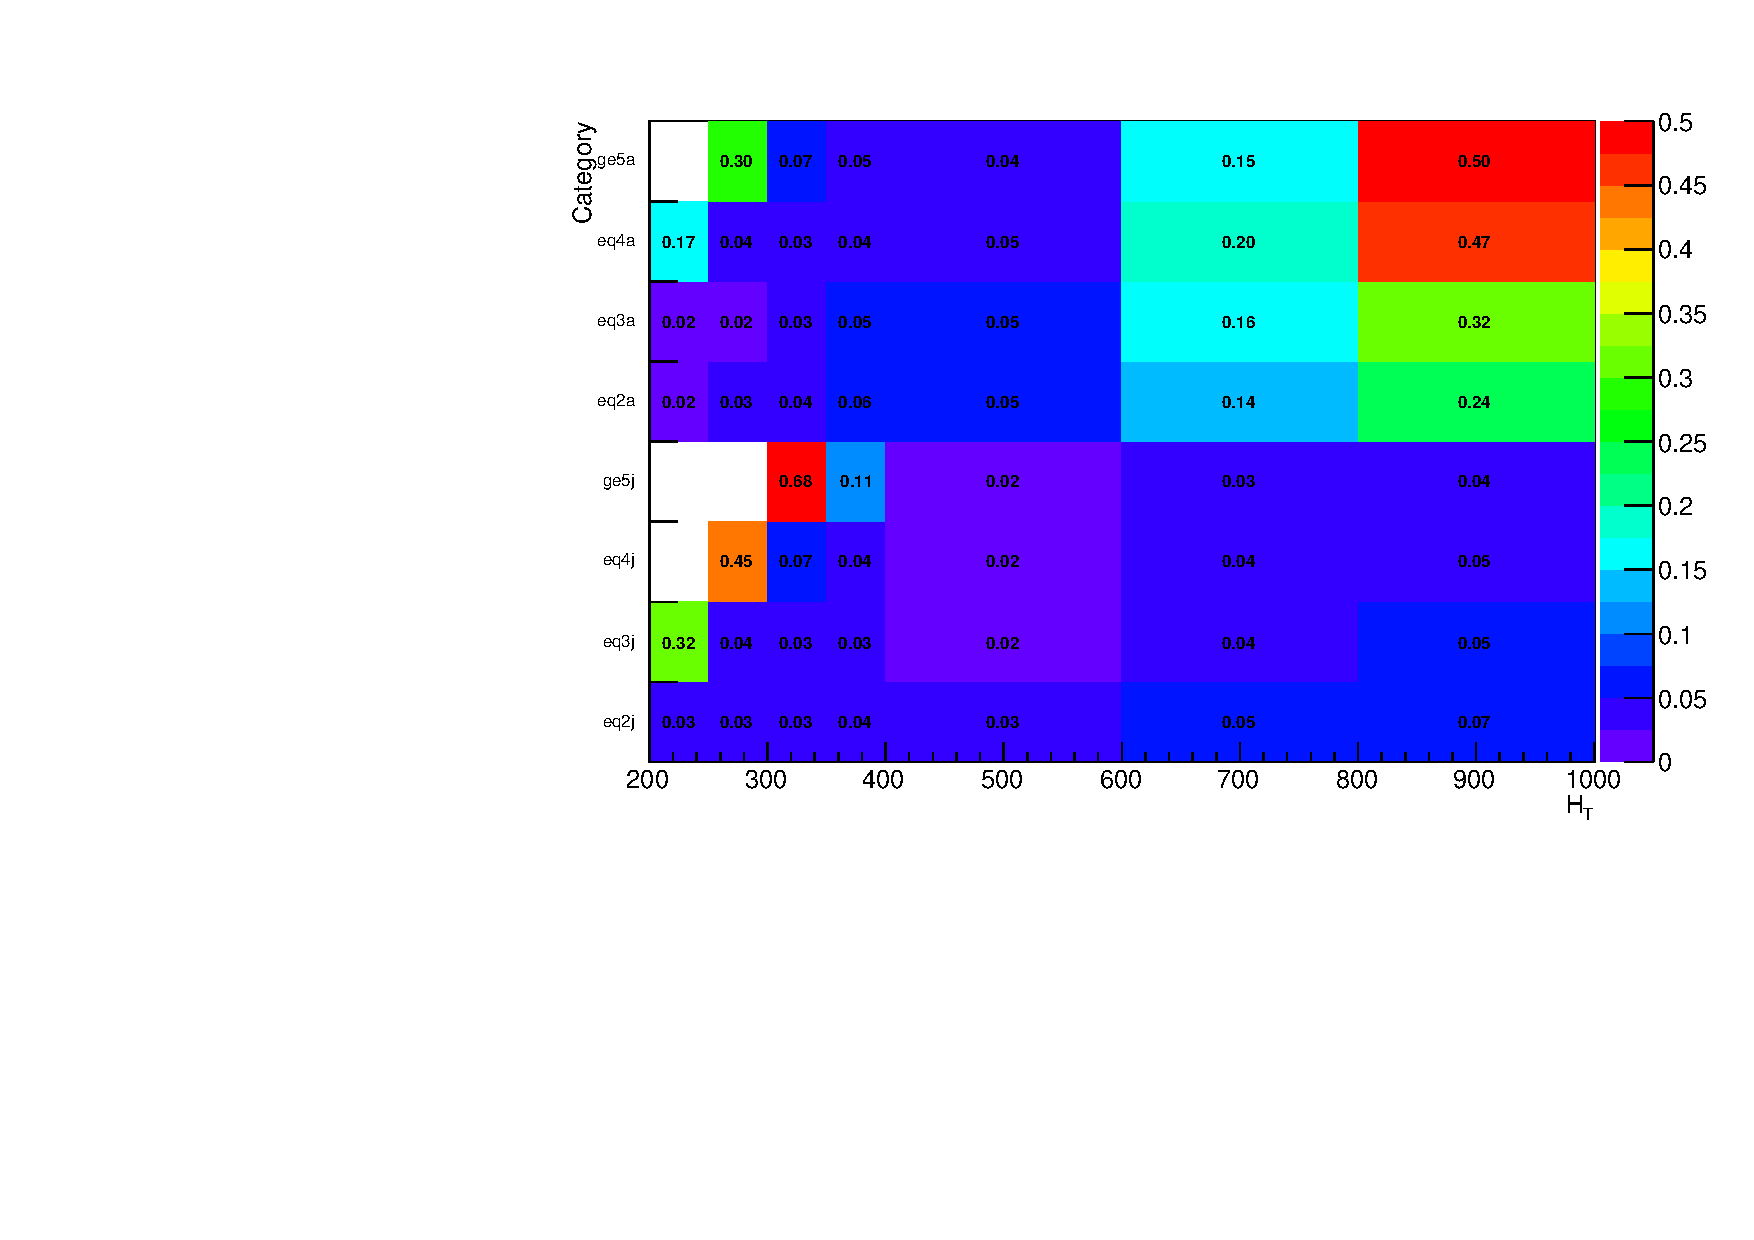
\includegraphics[width=0.5\textwidth]{figures/closureTests/systOut2d10fb.pdf}
  }
  \caption{\label{fig:systematics} Expected systematics derived from the closure tests shown for
the 3 \ifb and 10 \ifb scenarios}
\end{figure}

Finally, an additional dedicated study is used to determine the
systematic uncertainties that arise from uncertainties in scale factor
corrections related to b-tag modelling. These are generally found to
be small, at the percent level, and are typically sub-dominant with
respect to the systematic uncertainties derived from the closure
tests. However, if not sub-dominant, these additional uncertainties
are propagated through to the final total.

%% b jet multiplicity categories and also the seven \scalht regions,
%% which is a conservative approach given that one can expect some
%% correlation between adjacent \scalht bins (due to comparable
%% kinematics). This approach of decorrelating the \scalht regions
%% should be contrasted against the fits that do assume a correlated 
%% behaviour in \scalht.

\subsection{Systematic uncertainties in the \mht dimension\label{sec:syst-on-shape}}

The estimate of the number of events per (\njet,\nb,\scalht) bin,
integrated over \mht, is determined from data control samples, with
the associated systematic error determined from closure tests
described in Section \ref{sec:syst-from-closure}. This section
describes the method used to determine the systematic uncertainties in
how events are distributed according to \mht. 

Several potential sources of uncertainty will be considered, such as
ISR, JES, PDF, b-tag scale factors, etc, as detailed below. In
general, for each source of systematic, the \mht templates are found
based on $\pm$1$\sigma$ variations in the relevant source of
uncertainty. The alternative templates reflect the magnitude of the
migration of events between bins in \mht (but not in \njet, \nb, nor
\scalht, which is encapsulated by the normalisation systematic
uncertainties from closure tests). If the systematic source is found
to be significant, the template variations will be included in the
likelihood. 

An indicative behaviour is shown in Figure~\ref{fig:jec-shape} by
considering the variation of jet energy scale given the uncertainties
determined in Run~1. The relative change in the \mht distribution is
determined when varying the energy of all jets in an event up or down
according to a \pt- and $\eta$-dependent jet energy scale uncertainty
(\ie vary the event scale up and down), as recommended by the JetMET
POG. 

For the sensitivity studies reported in the AN, we assume a significant 
uncertainty on the distribution of events in the \mht dimension. 
At present this is modelled assuming a maximum of 50\% uncertainty in the last \mht bin, 
which typically represents the bin with the best single sensitivity in a given \scalht category. 
In this model the systematic uncertainty of lower \mht bins is determined 
as an exponential with a maximum shift of 50\% in the last \mht bin. 
Figure \ref{fig:mht-shape-syst-toy} shows the corresponding $\pm$1 Sigma variation of the 
\mht template obtained from this systematic model. 
As can be seen, this variation is much larger than the ones induced by MC variations (Figure \ref{fig:jec-shape}).  
We also have tested other models of the \mht systematic such as a linear instead of an exponential function which lead to rather similar results. 

\begin{figure}[]
  \centering
  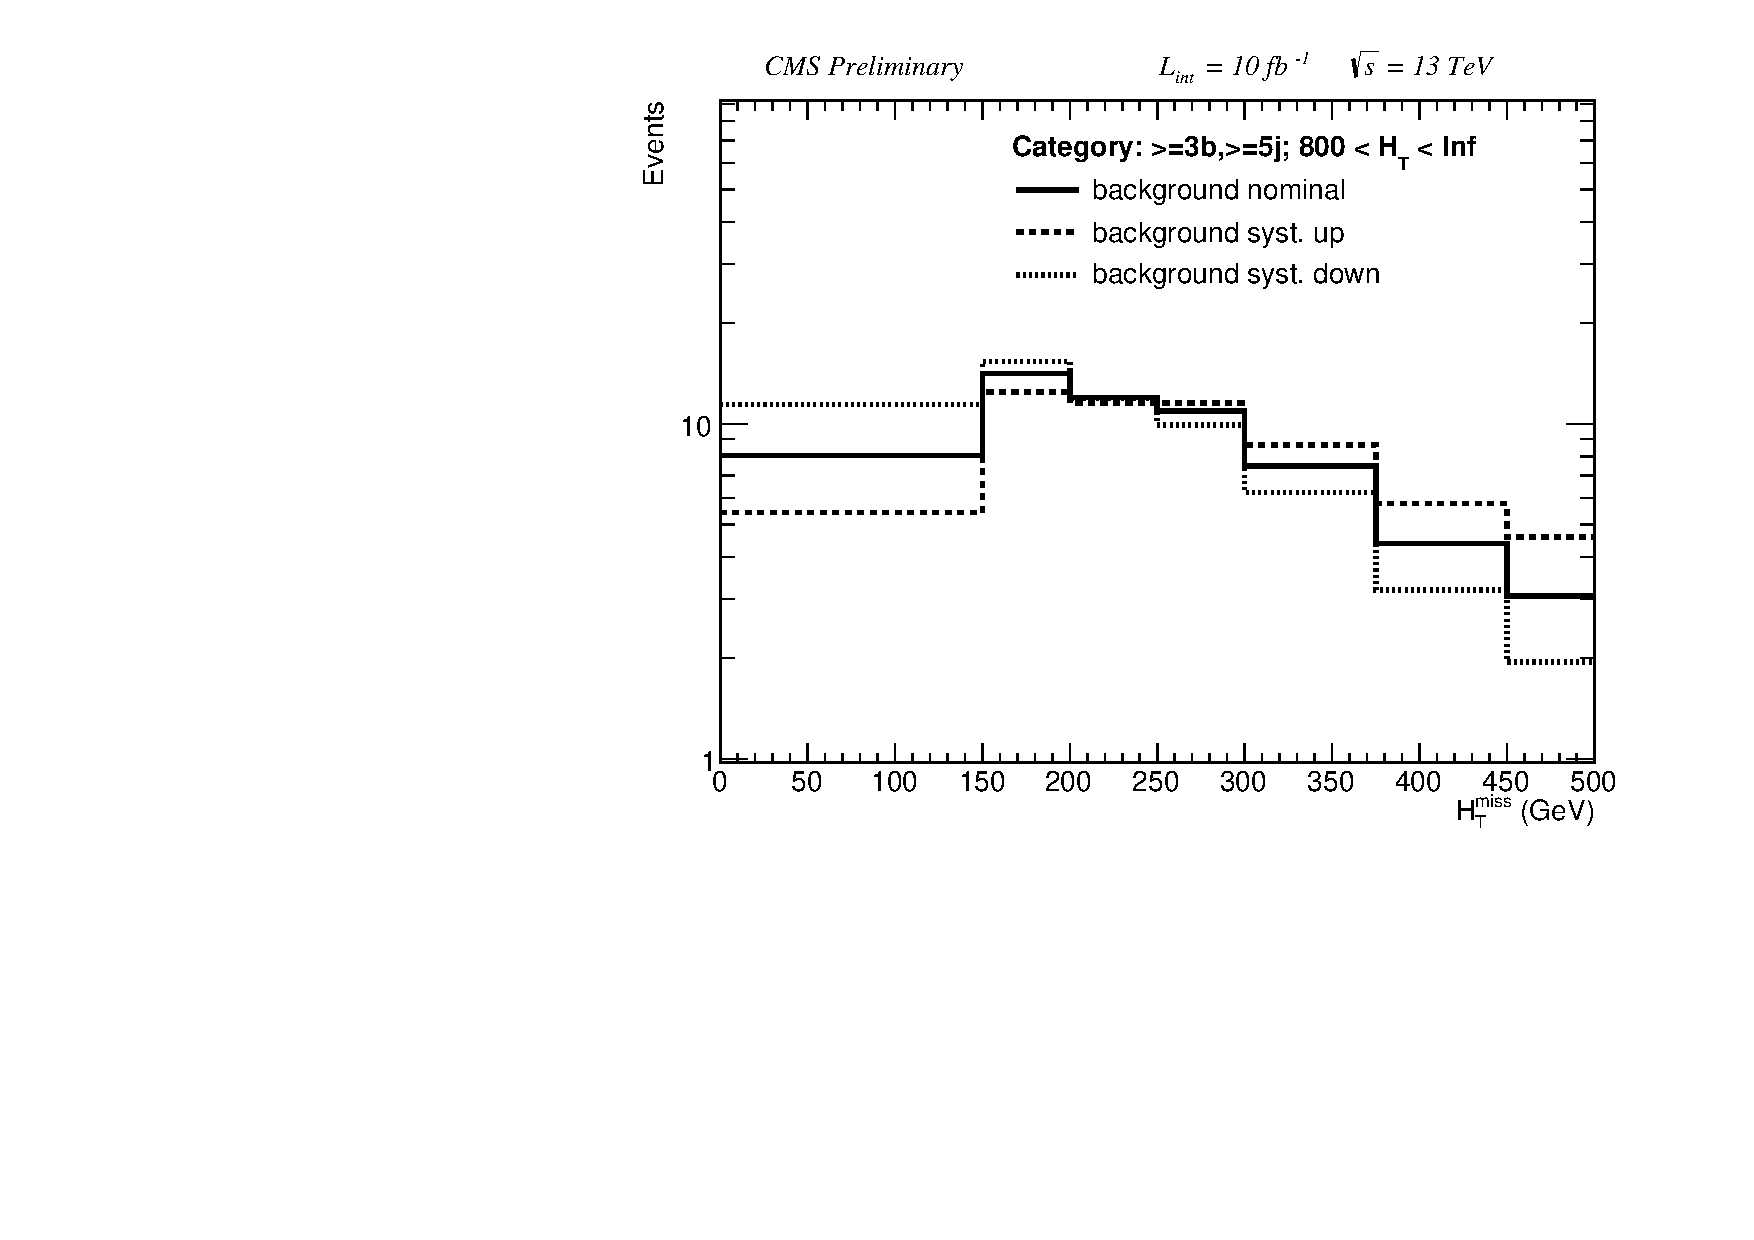
\includegraphics[width=0.7\textwidth]{figures/mhtShapeSyst/MHTShapeSyst_ge3b_ge5j_800_Inf.pdf}
  \caption{\label{fig:mht-shape-syst-toy} 
    The nominal \mht shape and its up/down alternative shapes for the $ttW$ background in the $\njet \geq5$, $\nb \geq 3$
    category for the $\HT > 800 \gev$ bin.
  }
\end{figure}

Finally, studies are underway with the aim of establishing procedures
based on data (akin to the closure tests) that will help to either
estimate dominant source of uncertainty related to how events are
distributed in \mht, or to at least provide data-driven cross checks.
An attempt to avoid a reliance solely on variations in simulation is
considered important for a discover-orientated analysis. The current
ongoing studies are based on Run~1 data.

%While simulation-based studies are also ongoing, some comments are
%made below on some of the potential sources of uncertainty that are
%expected to be dominant. This list is clearly not exhaustive.
%
%{\bf Jet energy scale:} 
%
\begin{figure}[]
  \centering
  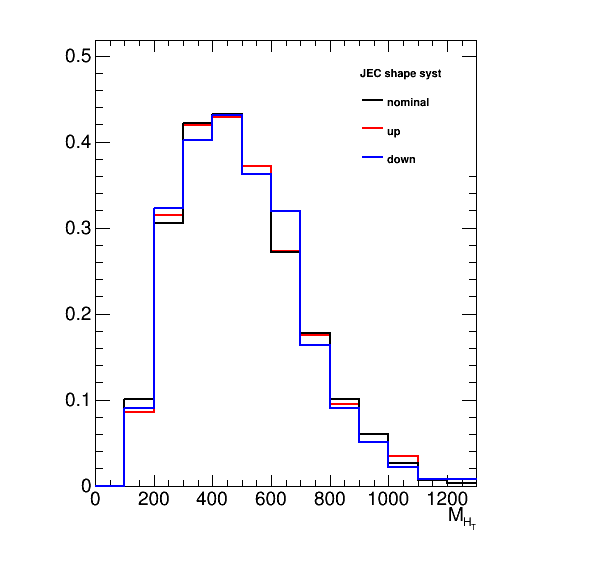
\includegraphics[width=0.5\textwidth]{figures/closureTests/mhtJetSyst_SMS_T1bbbb_2J_mGl1000_mLSP900_JEC_ge3b_ge5j_800_1600.png}
  \caption{\label{fig:jec-shape} Alternative \mht templates that
    refect uncertainties in the jet energy scale corrections for
    $\geq$5 jets, $\geq$3 b-jets, and $\scalht > 800\gev$ bin for the
    10 \ifb luminosity scenario.}
\end{figure}
%
%{\bf PDF uncertainties:}
%
%\newcommand{\lcr}{Left: $\frac{\epsilon_{CTEQ6L1}}{\epsilon_{CT10}}$,
%  center: $\frac{\epsilon_{CTEQ6L1}}{\epsilon_{MSTW08}}$, right:
%  $\frac{\epsilon_{CTEQ6L1}}{\epsilon_{NNPDF2.1}}$}
%
%The samples are produced with the \verb!CTEQ6L1! PDF set by default.
%The shape is compared with that obtained with three alternative PDF
%sets: \verb!CT10!, \verb!NNPDF2.1!, and \verb!MSTW2008!. The envelope
%and its uncertainties are determined following the PDF4LHC
%recommendation~\cite{pdf4lhc}. 
%
%{\bf Initial state radiation:}
%
%Will have to cook up a recipe for this\ldots
%
%
%{\bf \texorpdfstring{\mht/\met}{MHT/MET} cleaning cut:}
%
%The efficiencies for the requirement $\mht/\met < 1.25$ must be
%measured in data and simulation as a function of \mht for each \scalht
%bin. The ratio of these two efficiencies should be unity. Deviation
%from unity is taken to represent the uncertainties on the simulation
%modelling of this variable for processes with significant, genuine
%\met. This can be used to define templates for the uncertainty on this
%quantity.
%
%{\bf Dead ECAL filter:}
%
%The ratio of efficiencies observed in data and simulation for the dead
%ECAL filter may be used as in Section~\ref{sec:sms-syst-mht-met} to
%templates for the uncertainty from the Dead ECAL filter.
